% This is samplepaper.tex, a sample chapter demonstrating the
% LLNCS macro package for Springer Computer Science proceedings;
% Version 2.20 of 2017/10/04
%
\documentclass[runningheads]{llncs}
%
\usepackage{graphicx}
\usepackage{hyperref}
\usepackage{cleveref}
\usepackage{float}
\usepackage{textcomp}
\usepackage{caption}
\usepackage{subcaption}
\usepackage{listings}

\lstset{
language=C,
basicstyle=\small\sffamily,
numbers=left,
numberstyle=\tiny,
frame=tb,
columns=fullflexible,
showstringspaces=false
}

\captionsetup{compatibility=false}

\setcounter{secnumdepth}{3}
\begin{document}
%
\title{Smart Lecture Rooms at Universities}

\author{Group ID 07: Yunxuan Li \and
Jingxi Zhang \and
Zhixian Li}

\institute{Service Computing Department, IAAS, University of Stuttgart
\email{st119871,st141130,st146584@stud.uni-stuttgart.de}}
%
\maketitle              % typeset the header of the contribution
%
\begin{abstract}
This project is part of the lecture smart cities and internet of things \cite{ref_url1}. A lecture room is the most often and common place that student will go in an university. However, it is not easy to keep everyone in a lecture room comfortable, health and productive while have the lecture room itself secure and energy efficient. To achieve this goal, we plan to develop a smart lecture room system that uses different sensors to monitor the current state of a lecture room and automatically make decisions based on the information it has gathered.

\keywords{Lecture Room  \and Smart Building \and Comfortable \and Energy Efficiency \and AI Planning \and Cloud}
\end{abstract}
%
%
%
\section{System Introduction}
For students, a lecture room might be the most often place we stay in an university. However, it’s hard to have everyone comfortable in a lecture room, for example, someone might want to have fresh air, but it could be too cold for others. In addition, it would be hard to keep everyone productive, for example, there might be a reflection on black board, but the professor did not notice. Furthermore, it could also be hard to keep the security and energy efficiency of a lecture room, for example, the door of a lecture could be left open and the light of a lecture room could be left on after a lecture is done. Besides, it is not necessary to run the HVAC devices at full capacity if the room is not occupied. Therefore, we want to develop a smart lecture room system that not only tries to make everyone in the room comfortable and productive but also keeps the lecture room secure and energy efficient. \\
To accomplish this goal, we decided to use different sensors in a lecture room that monitor the temperature, the weather, the air quality and so on. Based on these sensors, we will develop an automate system that decides when to make actions such like open the window or close the light. Also, with the use of calendar data the system is able to plan ahead to schedule the heating device or open the doors. Unfortunately, the system cannot carry out all these actions automatically due to limited hardware support. Thus, the decision will be sent to the professor or the room management so that they can do the corresponding actions.

\section{System Analysis}
We will describe the system functionality using user stories in the following, where these user stories will be the main focus of our project.
\begin{itemize}
\item As a lecturer I want the room to automatically adjust light and curtains, so that my powerpoint is clearly visible.
\item As a student or a lecturer I want the room temperature and humidity to be as ideal as possible for a lecture.
\item As a manager of the cost of the buildings I want the system to idealize the energy so that the cost is minimized.
\end{itemize}
 
These two user stories involve a door lock. As a physical door lock with electric mechanism is expensive we will stick to a simplification like sending an email or using a light to indicate the state of the door.
\begin{itemize}
\item As a caretaker of the building I want the doors to be locked after lecture hours so that the security of the building is able to be guaranteed. 
\item As a student I want the doors to be open before lecture to be able to prepare my utils for the lecture.\\
\end{itemize}

\section{System Architecture Design}
This section describes our system architecture of our project which is depicted in \cref{fig:SystemArchitecture}.
The system's architecture is divided into four layers, (1) the \textit{physical layer}, (2) the \textit{ubiquitous layer}, (3) the \textit{reasoning layer}, and (4) the \textit{user layer}.
The components interact with each other via HTTP.

\begin{figure}[H]
\centering
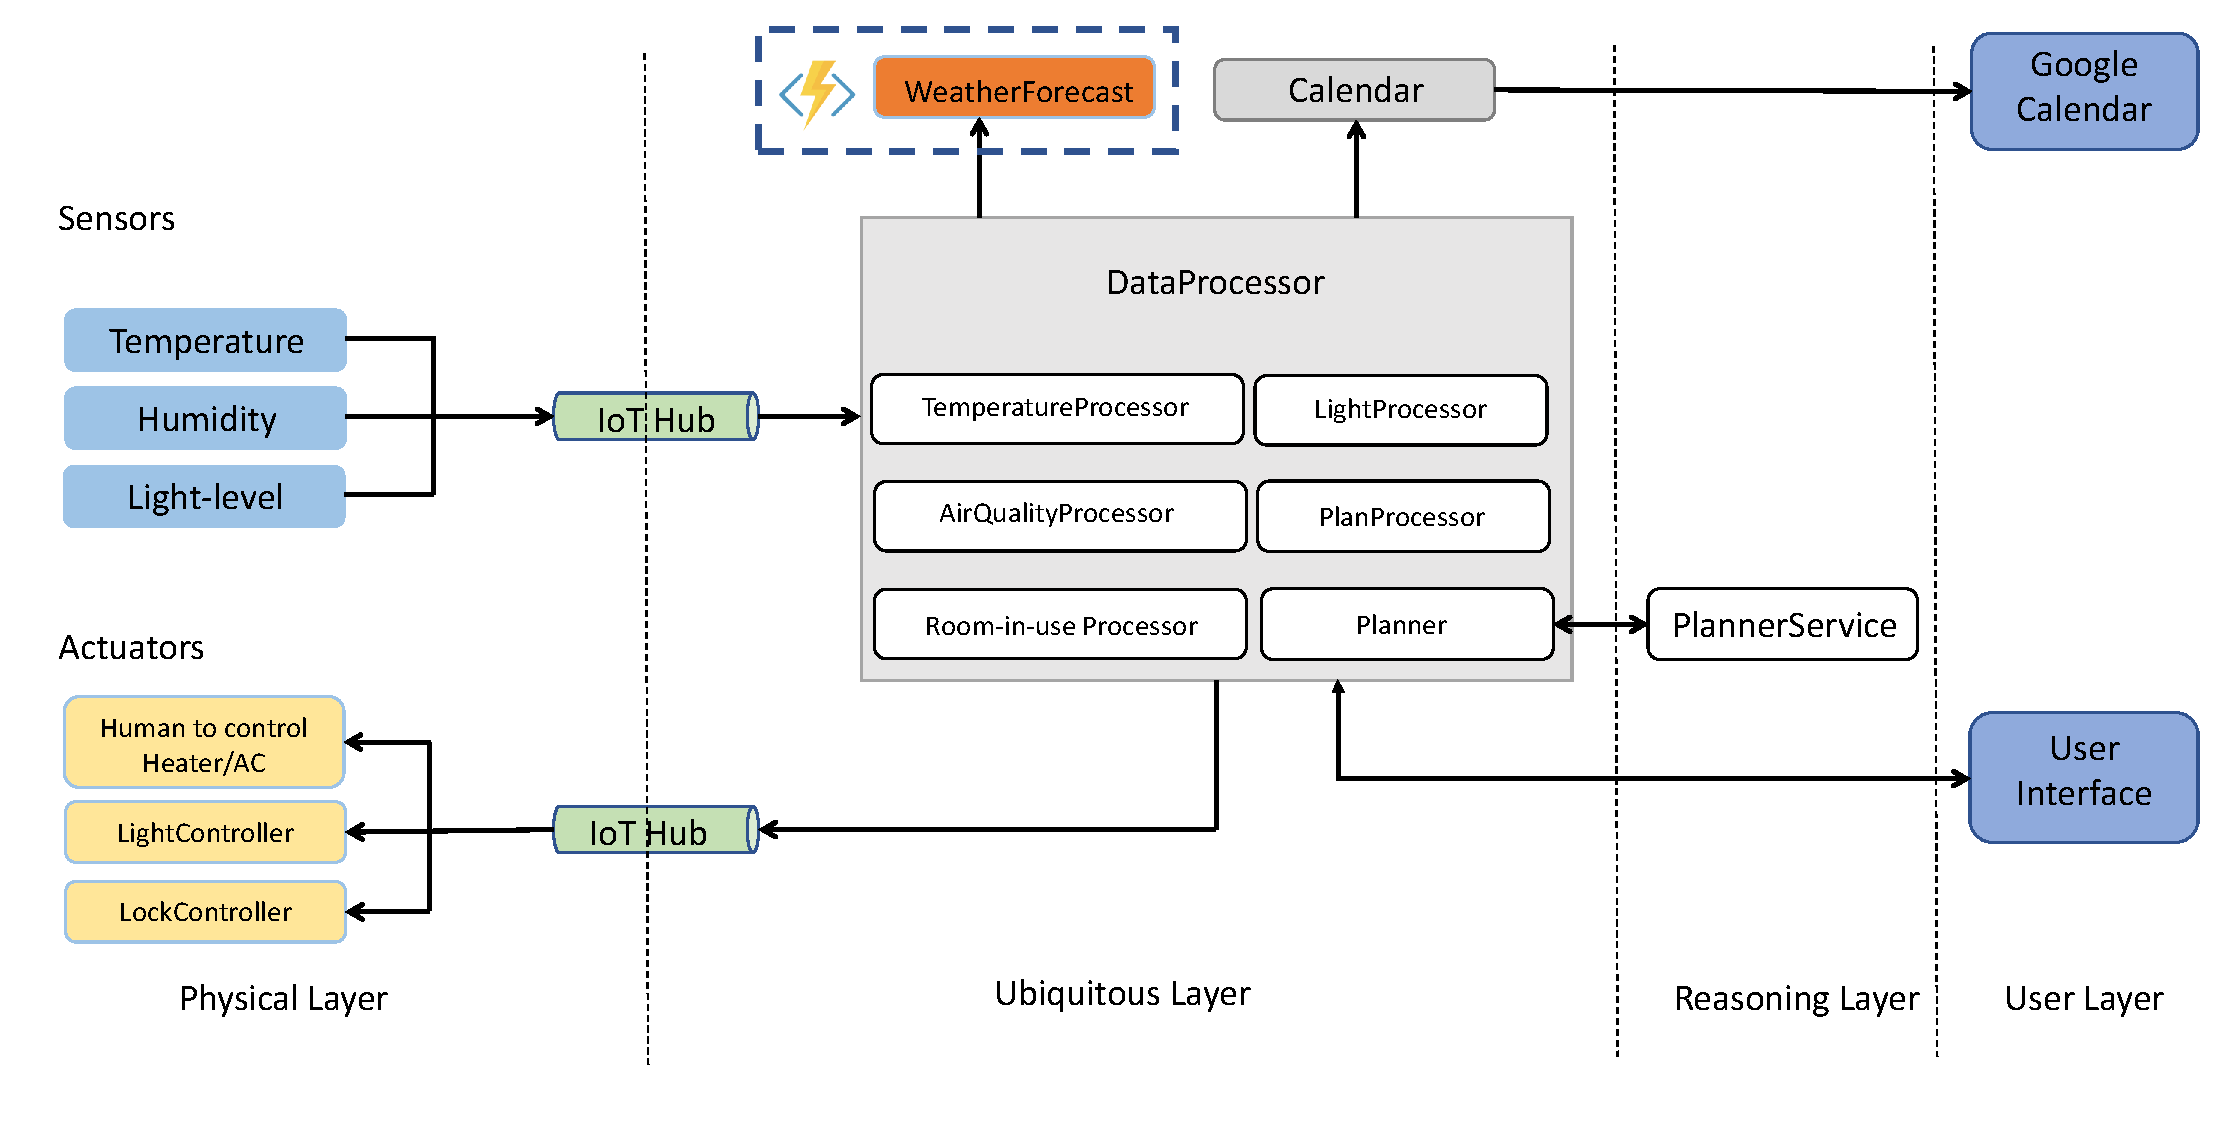
\includegraphics[width=1.0\textwidth]{../img/SystemArchitecture.pdf}
\caption{SystemArchitecture}
\label{fig:SystemArchitecture}
\end{figure}

The physical layer contains the components which are interacting with their physical environment.
There are two kinds of components, sensor components which are retrieving the sensor data for our project, and actuator components which are performing actions on their surrounding area to controll the temperature and light.
As sensor data we collect the temperature, humidity and light level of the lecture room via sensors on a Raspberri Pi.
They are sent to the ubiquitous layer though a gateway.
The actuators on the other hand serve as consumers in the physical layer.
They receive commands to be executed from the ubiquitous layer via another gateway and adapt the environment according to the commands.
As actuators we have a \texttt{LightController}, which is supposed to switch the light of the room off and on and to adjust the intensity of the light, i.e. the light level.
The \texttt{LockController} can lock and unlock the door of the room according to the calendar, so that outside of the allowed booking times nobody is allowed to enter the room without additional access authorization, like a key.
Furthermore a Heating Device should be controlled by the overall system.
For this purpose, a Smart Home thermostat could be used, which can operate the heating and is controlled by an application.
However, due to a lack of hardware, this cannot be implemented within the scope of this project.
For this reason the system is dependent on human help.
The same applies to the activation, deactivation and adjustment of the air conditioning system.
\texttt{LightController} and \texttt{LockController} are deployed on a Raspberry Pi.

The ubiquitous layer is the heart of the application.
It consists of the components \texttt{DataProcessor}, \texttt{Calendar}, and \texttt{WeatherForecast}.
The \texttt{DataProcessor} receives the sensor data from the sensors via a gateway and processes them.
For the weather forecast for the next 24 hours the \texttt{DataProcessor} calls the \texttt{WeatherForecast} component, which runs as \textit{Azure Function}~\cite{AzureFun50:online} in the Microsoft Azure Cloud.
The function gets the data for the location of the lecture room from \url{weatherbit.io} and returns the forecast.
In addition to sensor and weather data, the \texttt{DataProcessor} also retrieves calendar events for the room from the \texttt{Calendar} component, which retrieves the data via the \textit{Google Calendar API}~\cite{APIRefer59:online} from the Google Calendar of the room in which the lecturers entered them.
All data is then sent by the \texttt{DataProcessor} to the reasoning layer, where it is further processed by the \texttt{PlannerService}.
As a result of the processing, the \texttt{DataProcessor} receives a plan with actions to be performed, which it sends to the actuators via another gateway.

Our \texttt{PlannerService} at the reasoning layer is the part where \textit{AI Planning} comes into play. 
As described, it receives data about the environment from \texttt{DataProcessor} and makes a decision based on it using a \textit{PDDL Solver} in the cloud~\cite{solverpl71:online} as planner.
The cloud solver is called via an HTTP request. 

The user layer insists on the interaction of the lecturers with the Google Calendar, as well as a \texttt{User Interface}, in which the light and air conditions can be adjusted manually.


\section{System Implementation}
\label{sec:imp}
% Describe the implementation of your system. This section is only relevant for the report and should be omitted for the project description. 
The implementation of our project is divided into hardware implementation and software implementation. In the following, we will first describe the hardware implementation in \ref{imp:hard_imp} and then describe the software implementation in \ref{imp:soft_imp}.

\subsection{Hardware Implementation}
\label{imp:hard_imp}
The whole project is based on Raspberry Pi 3 Modell B Plus~\cite{pi3}. The complete demo looks like in picture \ref{pic:demo}. This demo can be seen as two parts. The first part is the Raspberry Pi 3 and the second part is the demo classroom with sensor and actuator connected to Raspberry Pi 3 through a breadboard. In this demo, we simulate a classroom with one window (actuator) and curtain (virtual), one door (actuator), three lights (actuator), a heater (virtual), a cooler (virtual) and with a temperature sensor (hardware), a humidity sensor (hardware), a light sensor (hardware), a weather source (website) and a calendar source (website). Because of the limitation of hardware, only the window, the door and three lights can be controlled by ourselves, all other apparat are considered to be virtual and we assume that the manager of the classroom has access to that. Thus, to control those virtual apparats, we will inform the manager instead of controlling it directly through Raspberry Pi 3.

\begin{figure}[H]
\centering
\includegraphics[width=0.6\textwidth]{img/demo}
\caption{Complete Demo} 
\label{pic:demo}
\end{figure}

In the following, we will first shortly explain each apparat that is used in this demo and then describe how it is connected to Raspberry Pi 3. As we used hardware sensor and software sensor in this project, we will only introduce the hardware sensors that are used in the project in this section. For information of how we gathered data from website, please refer to section \ref{soft_imp:sensor}

\subsubsection{Raspberry Pi 3 Modell B Plus}\hfill
\label{hard_imp:pi3}
\newline
We used Raspberry Pi as our core calculation and control part. The reason for that is Raspberry Pi is a very cheap computer that runs Linux and we currently have one in hand. Another advantage of Raspberry Pi over traditional computer is that it provides a set of general-purpose input/output(GPIO) pins that allow us to control electronic components such as temperature sensors or different actuators.

\subsubsection{Hardware Sensors}\hfill
\label{hard_imp:sensor}
\newline
The hardware sensors that are used in our project are listed below.
\newline
\textbf{Temperature and humidity sensor~\cite{th_sensor}}\\
For temperature and humidity, we found DHT11 sensor very useful as this sensor can provide us data of temperature and humidity at the same time. Furthermore, we found that the measurement range and accuracy of DHT11 is~\cite{th_data}:
\begin{itemize}
\item Temperature Range: 0-50 \textdegree{}C
\item Temperature Accuracy: $\pm$2\% \textdegree{}C 
\item Humidity Range: 20-90\% RH
\item Humidity Accuracy: $\pm$5\% RH
\end{itemize}
which is also suitable for our purpose. To connect DHT11 to our Raspberry Pi 3 we followed this tutorial~\cite{th_tutorial}. In our demo, we have connected DHT11 to pin 13 which corresponds to GPIO27.
\newline
\textbf{Light sensor~\cite{l_sensor}}\\
For light sensor, we used the light sensor from kwmobile. The data gathered from this light sensor is the resistance of the light-dependent resistor. The relation between the resistance and the brightness is that: the brighter the lights, the smaller the resistance.

To connect this light sensor to our Raspberry Pi 3 we followed this tutorial~\cite{l_tutorial}. In our demo, we have connected the light sensor to pin 7 which corresponds to GPIO4.

\subsubsection{Hardware Actuator}\hfill
\label{hard_imp:actuator}
\newline
The hardware actuators that are used in our project are listed below.
\newline
\textbf{Servo motor for window and door~\cite{m_actuator}}\\
To simulate the window and door we used two servo motors respectively. Both motors are Servo Motor, the difference between the implementation of being a window and a door is that, for window we let the motor rotate from the middle as shown in figure \ref{pic:window}, and for door we let the motor rotate from the lift side as shown in figure \ref{pic:door}. 
\begin{figure}[H]
\centering
\begin{subfigure}{.5\textwidth}
  \centering
  \includegraphics[width=.9\linewidth]{img/window}
  \caption{Servo motor for window}
  \label{pic:window}
\end{subfigure}%
\begin{subfigure}{.5\textwidth}
  \centering
  \includegraphics[width=.9\linewidth]{img/door}
  \caption{Servo motor for door}
  \label{pic:door}
\end{subfigure}
\caption{Servo motor for window(a) and door(b)}
\label{pic:sm}
\end{figure}

To connect both servo motor to our Raspberry Pi 3 we followed this tutorial~\cite{m_tutorial}. In our demo, we have connected the servo motor for window to pin 13 which corresponds to GPIO27 and we have connected the servo motor for door to pin 18 which corresponds to GPIO24.
\newline
\textbf{LED as lights}\\
To simulate the lights in a classroom we used three white LEDs as in a real classroom there are also multiple light sources. The LED we are using is just the most common LED from the market as we don’t have any other better hardware for lights.

To connect LED to our Raspberry Pi 3 we followed this tutorial~\cite{led_tutorial}. As in the tutorial, we also used a resistor in each LED circuit. This resistor can be moved away but the LED light will then be too brighter. In our demo, we have connected three LEDs (from right to left) to pin 29 (GPIO5), pin 31 (GPIO6) and pin 33 (GPIO13) respectively.

\subsection{Software Implementation}
\label{imp:soft_imp}

\subsubsection{Gather Data from Internet Sources}\hfill
\label{soft_imp:sensor}
\newline
Since our project needs the hourly weather forecast for the next 24 hours, it is necessary to use a weather service that can provide this data for a specific location via an API.
We decided to use \url{weatherbit.io} for this purpose, as the provider meets our requirements.
Weatherbit offers several API endpoints, including the current weather and the weather forecast we use.
In order to use the API of weatherbit, an API key is required, which is provided after account creation and selection of a service plan.
For our project the free plan is sufficient.
To ensure scalability and elasticity, the \texttt{WeatherForecast} component was implemented as \textit{Azure Function} in TypeScript, which can also be executed locally via the corresponding VisualStudio Code Extension.
The function can then call the weather forecast API endpoint with a \texttt{GET} request to \texttt{https://api.weatherbit.io/v2.0/forecast/hourly}.
The request must contain the location, the number of hours and the API key as query.
The weather data is returned in JSON format.

Besides, to plan ahead to open and lock the door or schedule the heating device and air conditioner we need the calendar data of the corresponding room. 
The Google Calendar API~\cite{APIRefer59:online} offers an API endpoint to retrieve calendar events via HTTP call.
First, however, the \texttt{Calendar} component must authenticate to the Google Calendar API via OAuth.
To do this, you must first enable the API for an account.
Activating it will provide you with credentials that must be specified during authentication.
If the authentication is successful, the \texttt{Calendar} component will receive an access token that allows the component to access the events of the calendar via the API. 
The component is implemented as an Express Server in Node.js and provides an endpoint for the components of the system to query the next 10 events in the room, which are then returned in JSON format.
Similar to the \texttt{WeatherForecast} component, the \texttt{Calendar} component can be deployed to the Microsoft Azure in a few steps through a VisualStudio code extension.
However, the \textit{Web App} service of Microsoft Azure is used for this purpose~\cite{WebAppDi86:online}.
Alternatively, the component can be installed locally or on any VM, provided the environment supports node version 12 or higher.

\subsubsection{Inform Human Actuator}\hfill
\label{soft_imp:actuator}
\newline
As mentioned in \ref{imp:hard_imp}, we have assumed some apparat such as curtain, cooler and heater to be controlled by the classroom manager. Thus, we need a method to inform the human actuator, namely the classroom manager.

To do so, we decided to inform the classroom manager through emails. The reason for that is, it is a cost-free action and it is easier to implement through python. When we are implementing the project, we also considered to used Whatsapp message, as we thought it would be more convenient and efficient than email. However, when we were exploring how to send messages through python, we notice that Whatsapp needs a more complexed authentication method (through python) and other tools that charges for each message sent. Hence, we decided to just use email to inform the classroom manager.\\

For our project, we registered a new email account: \url{noreply.scaiot.project@gmail.com}. All emails that needs to be send to the classroom manager will be sent from this email. To actually send the email to the classroom manager we used following code:
\begin{lstlisting}[language=python]
def sendEmail(receiver_email, content, subject="Information from scaiot project",
              sender_email="noreply.scaiot.project@gmail.com",
              password="xxxxxxxxxxx"):
    message = MIMEMultipart()
    message["Subject"] = subject
    message["From"] = sender_email
    message["To"] = receiver_email
    message.attach(MIMEText(content, "plain"))

    port = 587  # For starttls
    smtp_server = "smtp.gmail.com"
    context = ssl.create_default_context()

    with smtplib.SMTP(smtp_server, port) as server:
        server.ehlo()  
        server.starttls(context=context)
        server.ehlo()  
        server.login(sender_email, password)
        server.sendmail(sender_email, receiver_email, message.as_string())
\end{lstlisting}
In this function, we first use code from line 4 to 8 to generate the subject and content of an email and then use code from line 14 to 19 to open an TLS channal to send the email.


\subsubsection{AI Planing}\hfill
\label{soft_imp:ai}
\newline
For AI planing part, we decided on solver.planning.domains as it is the most simple one to connect. We also evaluated FastForward (\url{fai.cs.uni-saarland.de/hoffmann/ff.html}) as well as FF-Metric and its different extensions. 
They provide some functionality which would be needed, but are too much focused on one version of PDDL. The basic FF did not contain fluents which are needed for our comparisons of temperature and light. 
Another tool we looked at was SMTPlan+. This has too many dependencies and cannot be used on any machine. It also runs until an output is generated. So if there is no plan at all it expands any possible combination of actions until all are tested. This needs too much time to plan our domain and problem. \\
In the end the decision is the solver.planning.domains. They also provide a piece of python code to connect to their solver. The response is a json string which contains if the status was ok, an error or no response at all.
This string contains all the information we need to solve our problem. \\
We need the predicate "(output-done ?r)" to get an output in plan. As it cannot use less than or larger than comparisons as goal. In the following we will look into details of the domain and the problem.\\
\newline
\textbf{Domain formulation}\\
We need to refomulate the situation of our room into a domain. 
Our lecture room has at least a front door which can be closed and locked or open and unlocked. It also has an arbitary number of windows and curtains which are open or closed. The lights have three states off, dimmed or fully on. We also included the heater and air conditioner, but we need a human to turn them on and off as we do not have a phisical device for them. There is a predicate if the presenter is used or not.
\newline
Predicate if we are having a presentation in room:
\begin{lstlisting}
(presentingInRoom ?r - room)
(notpresentingInRoom ?r - room)
\end{lstlisting}
An example code for our window in domain:
\begin{lstlisting}
(are_closed ?win - window)
(are_open ?win - window)
\end{lstlisting}
There also needs to be a relation to the room:
\begin{lstlisting}
(has_window ?r - room ?win - window) ;room has windows
\end{lstlisting}
Then there are functions to input the temperature, the desired temperature and the outside temperature. They need the fluents package.
Another value is the lightlevel. Here we also have a desired value as well as a actual value. These functions are used to compare the values.\\ 
\newline
For each possible real action we added an action in the domain. \\
Let us start discussing the door actions. Its states are open and closed. To switch states it needs two actions. One to close it and one to open it. \\
The opening is dependent on whether there will be the first lecture of the day in the room. It also needs the state of the door which is closed. The effect will be the unlocking of the door. \\
The closing is dependent on whether the lecture time is over and whether there are people in the room. \\
\begin{lstlisting}
(:action unlockRoom ...)
(:action lockRoom ...)
\end{lstlisting}

Next let us look at light related actions. 
For these actions we need the curtain status and the light status. The light has three levels: off, dimmed and on.\\ 
We check if the light level inside the room is higher than the desired we need to turn down the lights. If it is lower we need to increase the brightness.\\ 

To decrease the brightness we first check if the curtains are down and try to lower them if they are up. But when they are already down we need to adjust the lights. From the state dimmed we can turn them to off and from on we can turn them to dimmed. \\
The following actions reflect the description:
\begin{lstlisting}
(:action curtain_down ...)
(:action dimLightsdown ...)
(:action lightsOff ...)
\end{lstlisting}
To increase brightness we check the curtain and the light status again. We can pull up the curtain if they are down. Then adjusting the lights from off to dimmed or from dimmed to fully on can change the light level. \\
These actions are responsible for turning up the light level.
\begin{lstlisting}
(:action curtain_up ...)
(:action dimLightsup ...)
(:action fullLights ...)
\end{lstlisting}
In the case none of the actions darkened/brightened the room, the lights or the sensor is defect.\\

The temperature and humidity are related with the windows, the heater and the air conditioner. \\
An action which is always done is refreshening the air between lectures. Here we need the humidity and the windows status. Inbetween lectures the following action takes place to regulate the air.
Conditions for the windows to open is the between lecture time, closed windows and the actual humidity in the room in comparison to the outside and the desired humidity. 
\begin{lstlisting}
;humidity related
    (:action refresh_air
        :parameters (?r - room ?o - outside ?win - window)
        :precondition (and
                        (betweenLectures ?r)
                        (has_window ?r ?win)
                        (are_closed ?win)
                        (or 
                        (and
                  (< (humidity_wanted ?r) (actual_hum ?r))
                  (> (actual_hum ?r) (outside_hum))
                        )
                        (and
                  (> (humidity_wanted ?r) (actual_hum ?r))
                  (< (actual_hum ?r) (outside_hum))
                        )
                      )
        )
        :effect (and
            (are_open ?win)
            (not (are_closed ?win))
            (output-done ?r)
        )
    )
\end{lstlisting}

While a lecture is going on our desired temperature is 24C. To accomplish this goal the windows and the heater and the air conditioner are used as follows.

If the temperature inside is higher than the desired one we need to distinguish between two cases which are related to the outside temperature. If we have a higher or equal temperature outside we need to use the air conditioner to lower the temperature inside to 24C. But if the outside temperature is lower than the inside temperature we open the windows. This we we can avoid using the air conditioner all the time and safe energy.
\begin{lstlisting}
(:action open_Windows ...)
(:action cooler_On ...)
\end{lstlisting}
If we reached our desired temperature and the windows are still open we close them. \\
In case the outside, the inside and the desired temperature are equal there is no need to take any action.
\begin{lstlisting}
(:action cooler_Off ...)
(:action close_Windows ...)
(:action heater_Off ...)
\end{lstlisting}
If the temperature inside is lower than the desired temperature, we also have two cases. If it is colder or equally cold outside as inside, we turn on the heater to reach our desired temperature. If it is warmer outside than inside and the desired temperature is higher than the inside temperature we can open the windows.
\begin{lstlisting}
(:action open_Windows ...)
(:action heater_On ...)
\end{lstlisting}
Following table reflects the rules described above, which are realized in the domain code. With o standing for outside temperature, i for inside temperature and d for desired temperature. ac stands for air conditioner.\\

\begin{tabular}{|c |c |c| c|c|c|}
\hline
case &o $>$ i $<$ d & o $\leq$ i $<$ d & o $=$ i $=$ d & o $\geq$ i $>$ d & o$ <$ i $>$ d \\
\hline
action &open Window & heater on & nothing& ac on& open Window\\
\hline 
\end{tabular}\\

For the full domain file please refer to our github \url{https://github.com/Jinaz/scaiot-project/blob/master/Implementation/PDDL_DATA/domain.pddl}
\newline
\textbf{Problem formulation}\\
To use a solver we need a formulation of a problem(problem.pddl).
To create the problem we need the current status of our room.
The current status of the window, lights, curtain and door as well as the temperature, humidity, lightlevel and ir-values are written into the problem in the init part. The current weather depending on weather forecast and the current time with respect to whether it is a lecture are also added. 
The last bit are the desired values.\\
The PddlWriter puts these information together and fills out a template file. 
\newline
\textbf{Plan interpretation}\\
The plan received is interpreted in the pddlReader. This plan is the response on our domain and problem file. The plan is a json where we filter out the actions and build a list of actions from it. 
Now that we got a list of actions we just need to execute them.

\section{Discussion and Conclusions}
In this project, we implement a small demo that simulate a smart classroom situation. In this demo, the data of the environment is collected from both hardware sensors and online sources. After the data is collected, it was sent to an online AI planner with a given room status and problem definition. Finally, when the plan is calculated from the planner, the corresponding actions will be taken, or the manager will be informed.\\

The core function of a smart classroom is basically realized in out demo, however, there are some features that we wanted to include at the beginning of the project but are end up with not implemented. For example, one feature that is not implemented is to detect whether a beamer is on and if there is reflection on projector curtain and if so, the lights should be closed, and the curtain should be put down. We tried to implement this feature, but we found out that it is hard to detect whether a beamer is on with the hardware we have, and it is also not meaningful to assume that this information can be got from a calendar. Furthermore, the reflection on projector curtain is also hard to detect, as the reflection is also related to a viewer’s watching angle and cannot be detected by a single light sensor. In the AI Planning domain, we have presentation modelled, thus, when we have the corresponding hardware, we can then easily add this feature.\\

During the implementation, we also noticed that some places can be done better. For example, in our implementation we have a model that remembers the status of a classroom, however, a change of a status is triggered by the plan. This means, if a plan told us to open the window, we will then execute the window actuator to make it open and set the window status of the classroom to open. A problem might occur is that, when the actuator is broken or offline, the status will still be changed even though the action has not been taken. The reason for that is because we do not have corresponding hardware that can give us information of the status of a classroom (such as if a door or window is locked, if lights is on, etc.), so we have to keep the changes of status based on actions.\\

The biggest problem we have faced during the implementation is the lack of hardware and time limitation. Based on the resources we have, we successfully implemented a small demo that can collect data from sensors and online sources. It will then take corresponding actions from a AI Planning plan to achieve a given goal. To conclude, we are satisfied with the result we have achieved in the end and we think doing this project is a good opportunity to explore internet of things


%
% ---- Bibliography ----
%
\bibliographystyle{splncs04}
\bibliography{mybib}

All links were last followed on April 17, 2020.

\end{document}
